\documentclass[12pt]{report}
\usepackage{setspace}
\onehalfspacing

\usepackage{arxiv}

\usepackage[utf8x]{inputenc} % allow utf-8 input
\usepackage[T1]{fontenc}    % use 8-bit T1 fonts
\usepackage{hyperref}       % hyperlinks
\usepackage{url}            % simple URL typesetting
\usepackage{booktabs}       % professional-quality tables
\usepackage{amsfonts}       % blackboard math symbols
\usepackage{nicefrac}       % compact symbols for 1/2, etc.
\usepackage{microtype}      % microtypography
\usepackage{float}
\usepackage{amsmath} 
\usepackage{mathtools}
\usepackage{algorithm}% http://ctan.org/pkg/algorithms
\usepackage{algpseudocode}% http://ctan.org/pkg/algorithmicx
\usepackage{listings}
\usepackage{color}
\usepackage{tikz}
\usetikzlibrary{arrows,positioning,automata}
\lstset{language=C}

\newtheorem{example}{Example}
\newtheorem{definition}{Definition}[section]
\newcommand\pair[1]{\langle#1\rangle}
\newcommand\alg[1]{{\sc#1}}
\newcommand\tool[1]{{\sc #1}}
\newcommand\os[1]{{\textcolor{blue}{os:#1}}}
\newcommand\crjs[1]{\textcolor{purple}{[CRJS: #1]}}
\renewcommand\rule[1]{\scalebox{.8}{({\sc \lowercase{#1}})}}
\newcommand\premise[1]{\scalebox{.8}{{\sc \lowercase{#1}}}}
\newcommand\longversion[1]{#1}


\title{Thesis}

\author{
  Chaked R.J.~Sayedoff \\
  IE, Technion, Haifa, Israel.\\
    \texttt{chaked@campus.technion.ac.il}\\
}

\begin{document}

\maketitle



\begin{abstract}
Given two programs $p_1$ and $p_2$, typically two versions of the same program, the goal of \emph{regression verification} is to mark pairs of functions from $p_1$ and $p_2$ that are equivalent, given a definition of equivalence. The most common definition is that of \emph{partial equivalence}, namely that the two functions emit the same output if they are fed with the same input and they both terminate. 
The strategy used by the Regression Verification Tool (RVT) is to progress bottom up on the call graphs of $P_1,P_2$, abstract those functions that were already proven to be equivalent with uninterpreted functions, turn loops into recursion, and abstract the recursive calls also with uninterpreted functions. This enables it to create verification conditions in the form of small programs that are loop- and recursion-free. This method works well as long as the two compared functions are in sync, and typically fails otherwise. In this work we study the problem of proving equivalence when the two recursive functions are not in sync. Effectively we extend  previous work that studied this problem for functions with a single recursive call site, to the general case. We also introduce a method for detecting automatically the unrolling that is necessary for making two recursive functions synchronize, when possible. We show examples of pairs of functions with multiple recursive calls that can now be proven equivalent with our method, but cannot be proven equivalent with any other verification system.
\end{abstract}

\chapter*{Dedication}
To my beloved wife who supported me all along.


\chapter*{Acknowledgements}
This research was carried out under the supervision of Prof. Ofer Strichman as
part of the degree in Master of Science In Information Management Engineering
in the Faculty of Industrial Engineering and Management.
\vspace*{\fill}

The generous financial help of the Technion is gratefully acknowledged

\tableofcontents

\chapter{Introduction}

\section{Regression Verification}
It is very common that changes in program introduce new bugs. There are two dominant methods today aiming to ensure code quality. The first is a manual check of the code by the developer and its colleagues – also known as \emph{code review}. The other method is \emph{regression testing}. The developer creates a set of tests that describes the expected behavior of the program. Then, the code is checked against those tests whenever a new version is introduced. This method is not complete as there might be corner cases the test's writer have missed. Even in the case we have found an anomaly, debugging is usually an expensive action we had rather avoid. Godlin and Strichman have proposed a new approach named \emph{regression verification} \cite{DBLP:conf/dac/GodlinS09}. \emph{Program verification}, the challenge of automatically proving the correctness of a program with respect to a given specification, is an impossible task due to its undecidable nature. It was called a "grand challenge" by Hoare \cite{DBLP:journals/jacm/Hoare03}. Regression verification suggests verifying the program against an older version of itself rather than verifying it against a specification. That is, generate an automated proof of equivalence between a program and its previous version. For closely related programs, regression verification is believed to be easier in practice than program verification. It spares the need to manually specify a specification and it can use the similarity between the programs to reduce computational burden \cite{DBLP:conf/dac/GodlinS09}. The notion of the verification is weakened that way, as the last version might suffer from the same problems as the new one. Nevertheless, regression verification is relevant in the same places where regression testing is acceptable to ensure the code quality. Specifically, regression verification is most effective when the code has changed but supposes to behave the same toward its interfaces. This is true for \emph{refactoring}, where the code was rewritten to match a certain convention, and it's also true for \emph{performance tuning}. One might wonder what equivalence between program means, and this question has several answers indeed. In this article we will use the \emph{partial equivalence} notion \cite{DBLP:conf/dac/GodlinS09}. $P_1$ and $P_2$ are partially equivalent if upon the same input, terminated executions of both programs yield the same output. Hereon, any reference to equivalence will refer to partial equivalence.

\subsection{Various Approaches to Regression Verification}
We will show here several techniques that try to cope with the regression verification challenge.

REVE (stands for REgression VErification) \cite{DBLP:conf/kbse/FelsingGKRU14} aim to infer a coupling predicates for a pair of programs $P_1$ and $P_2$, which is an invariant that relates $P_1$ and $P_2$ throughout their execution. They steer its generation so it will imply equality of the results in the case where they both terminate. If such a predicate can be inferred, they have proven equivalence between $P_1$ and $P_2$. To do so they compose a predicate containing function summaries, which are expressed as Horn clauses, loop and recursion invariants, and expressions containing the \emph{weakest liberal precondition} ($wlp$) notion. the \emph{weakest precondition} was proposed by Dijekstra \cite{DBLP:journals/cacm/Dijkstra75}. \emph{wp($P,\varphi$)} denotes the weakest condition that needs to hold before an execution of statement list $P$ such that the execution terminates and the postcondition $\varphi$ holds in the final state. for \emph{wlp($P,\varphi$)} , it demands $\varphi$ will holds after the execution of the program $P$ only if $P$ terminates. The invariants are synthesized automatically. Empirically, when the programs are closely related it is enough to propose the equivalence of related variables in the context as the invariant. Then, they exhaustively use \emph{wlp calculus} to reduce the formula to a pure Horn clause. In the end they use a Horn constraint solver, such as Z3 \cite{DBLP:conf/sat/HoderB12} or Eldarica \cite{DBLP:conf/cav/RummerHK13}, to prove the equivalence or generate a counter example upon non-equivalence.

SYMDIFF by Microsoft \cite{DBLP:conf/cav/LahiriHKR12} confronts this challenge from a different angle. Like REVE, it is most effective in cases of closely related programs. It concentrates on the \emph{conditional equivalence} notion which means that two programs are equivalent under a certain input condition. To do so, for each pair of functions it composes a procedure which assume the input condition, executes both function and asserts that their results are equal. The functions are flattened by replacing all functions invocations with calls to \emph{uninterpreted functions} (hereon will be referred as $UF$s), which are an abstraction of the original functions. A $UF$ returns a non-deterministic value for each input (sometimes some determinization is applied to preserve consistency). One may notice that a $UF$ is an over approximation of its corresponding function. SYMDIFF handle loops by transforming them to tail-recursive functions. Iteratively, SYMDIFF assumes the functions are equal and try to prove it using the SMT Solver Z3. In the case of failure, it takes the counter example produced by Z3, refines its input condition and try to prove again. It does so until settling on a fixed-point and then it will return the input condition upon it the programs are partial equal.

TODO:Write about tools using symbolic execution such as ModDiff, CLEVER, DSE (Differential Symbolic Execution) and IMP-S (IMPacted Summaries)

It is worth mentioning that every verification tool such as SeaHorn \cite{DBLP:conf/cav/GurfinkelKKN15}, HSF(C) \cite{DBLP:conf/tacas/GrebenshchikovGLPR12} and Automizer \cite{DBLP:conf/cav/HeizmannHP13} can be used to prove equivalence between programs. It can be done by generating a new program which executes the given programs with the same non-deterministic input and asserts that their output is equal. However, this method does not take any advantage of any feature that the regression verification case offers. Both REVE and SYMDIFF perform better on closely related programs because they exploit the similarity to reduce the computational overhead. Since verification techniques run in an exponential complexity, using a regular verification tool without any optimization might yield insufficient results. 

\section{Weakest Precondition}
\label{sec:wp}
Write about Weakest Precondition \cite{10.1145/360933.360975}

\section{Thesis Outline}


\chapter{An Overview of RVT}
\label{sec:rvtreview}
\section{RVT's Strategy for Proving Equivalence}
RVT is a Regression Verification Tool, originally developed by Godlin and Strichman \cite{DBLP:conf/dac/GodlinS09}. RVT tries to prove partial equivalence for a pair of programs. Its strategy to solve the program equivalence challenge is inspired by the Hoare's rule for recursive invocation~\cite{DBLP:series/lnm/Hoare71}: 

\begin{equation} \label{eqn:parteq}
 {\frac {\{p\} call\ \emph{proc} \{q\} \vdash_H \{p\} \emph{proc}-body \{q\}}{\{p\} call\ \emph{proc} \{q\}}} 
  (PART-EQ) 
\end{equation}

The rule says that if we can assume that {p} holds before the call to the procedure \emph{proc} and {q} holds afterward, and using this assumption we can prove that if {p} holds before executing the procedure body \emph{proc-body} then {q} holds afterward, we can infer that if {p} holds before calling to \emph{proc} then it is granted that {q} will hold after the call, hence it is an inductive argument: using what we want to infer as a hypothesis for the proof. They introduced a new inference rule~\cite{DBLP:conf/dac/GodlinS09}, in the spirit of the one we saw above. For recursive functions $P1$ and $P2$ the rule is
\begin{equation}
 {\frac {{\emph{in}[call\ P_1]=\emph{in}[call\ P_2]\rightarrow \emph{out}[call\ P_1]=\emph{out}[call\ P_2]} \vdash{\emph{in}[P_1\ body]=\emph{in}[P_2\ body]\rightarrow \emph{out}[P_1\ body]=\emph{out}[P_2\ body]} }
{{\emph{in}[call\ P_1]=\emph{in}[call\ P_2]\rightarrow \emph{out}[call\ P_1]=\emph{out}[call\ P_2]}}} 
\end{equation}
Less formally, this rule states that if  assuming that $P1$ and $P2$ produce the same output for the same input enables us to prove that the same input yields the same output upon executing $P1$ and $P2$ bodies, then the congruence relation between $P1$ and $P2$ (i.e., equal input results in equal output), holds. It was implemented by replacing recursive calls with calls to uninterrupted functions – $UF$s. An $UF$, as we explained earlier, is an over approximation of the substituted function that returns a non-deterministic value. By replacing the recursive call in both $P1$ and $P2$ with $UF$s that are defined as equal we have fulfilled the first part of the hypothesis. Then, all is left to do is prove the second part in order to prove the equivalence of $P1$ and $P2$. To Prove this equivalence, RVT generates a program calling both programs with the same non-deterministic input and asserts their output is equal as can be seen in figure \ref{fig:rvtmainprogram}.
\begin{figure}[h]
\begin{center}
\begin{minipage}{7 cm}

\begin{lstlisting}
i = non_det()
res1 = P1(i)
res2 = P2(i)
assert(res1 == res2) 
\end{lstlisting}
\end{minipage}
\caption{RVT's Generated Verification Program}
\label{fig:rvtmainprogram}
\end{center}
\end{figure}
CBMC is used to prove this assertion or produce a counterexample in case of failure. CBMC is a bounded model checker. Given a C program (possibly annotated with assertions reflecting the user's specification), it tries to verify for various things such as memory safety, general exceptions, undefined behavior, user assertions and more. It does so by unwinding loops and recursions and creating a \emph{Static Single Assignment} SMT (or SAT) formula which in turn is passed to an SMT (or SAT) Solver. The Solver will either prove the generated specification up to a given unwinding depth, or produce a counterexample. 

\section{A Decomposition Algorithm For Program Equivalence}
All we have seen so far did not take any advantage of the similarity between the programs. RVT tries to exploit similarity between the two versions of the program. It aims for the complexity to be a function of the difference between the programs rather than their absolute sizes. To do so it uses the decomposition algorithm that is presented in Algorithm \ref{alg:Prove}. \alg{Prove} receives a pair of programs $P$ and $P'$ and a (optionally partial) mapping between the functions in each program. RVT processes these programs before sending them to \alg{Prove}. All loops are transformed to recursive functions~\cite{DBLP:conf/vstte/StrichmanG05}. The recursive calls are then replaced with uninterpreted functions, hence making the program abstract and `flat', i.e., no loops and recursions. The problem of verifying flat programs is decidable. 

RVT also creates $map_f$ before sending it to \alg{Prove}, starting with all the obvious mappings – identical functions and global variables with the same name. Then, recursively, it advances on the parse tree of both programs and tries to map more elements (such as variables, functions and types) in isomorphic locations. It is important to note that wrong mapping cannot damage the soundness of \alg{Prove}, just its completeness. 
\alg{Prove} start by inlining nonrecursive nonmapped functions. Then it generates two graphs $MD_1$ and $MD_2$ where their nodes are the maximal strongly connected components (MSCC) in the call graphs of $P$ and $P'$. Because of the definition of MSCC, $MD_1$ and $MD_2$ are acyclic. After the setup in lines \ref{step:inline}-\ref{step:possible}, it starts traversing $MD_1$ and $MD_2$ bottom-up. Every MSCC is either trivial (i.e., a nonrecursive function) or nontrivial (i.e. one or more functions in a call cycle). When it encounters a pair of trivial MSCCs it checks for equivalence and marks it as equivalent if it manages to prove it (lines \ref{step:m1}-\ref{step:m1endIf}). If a pair of nontrivial MSCCs was encountered, a set $S$ of function pairs that their functions intersect all cycles in both MSCCs is chosen. Equivalence is checked for each of those pairs. In case of failure on any of the pairs, RVT aborts. That is because once RVT cannot prove equivalence for a recursive function (or mutually recursive functions) it cannot proceed proving any of its ancestors. This differs from the trivial MSCC case as functions in trivial MSCCs that RVT could not prove to be equal can be inlined in their ancestors when checking for their equivalence. In case of complete success (i.e., all the pairs in $S$ were proved equivalent), RVT marks all the pairs in $S$ as equivalent (lines \ref{step:select}-\ref{step:selectEnd}). Then the MSCC pair is marked as covered and RVT continues to the next mapped pair (line \ref{step:mark}).

\begin{algorithm}
\begin{algorithmic}[1]
\Function{Prove}{Programs $P,P'$, map between functions $map_f$}
\State \label{step:inline} Inline nonrecursive nonmapped functions;
\State \label{step:generate} Generate MSCC DAGs $MD_1, MD_2$
          from the call graphs of $P,P'$;
\State If possible,\label{step:possible} generate a bijective map $map_m$ between nontrivial nodes in $MD_1$ and $MD_2$ that is consistent with 
\mbox{~~~~~} $map_f$ (it is desirable but not necessary to add pairs of trivial nodes to $map_m$). Otherwise abort.
\While {$\exists \pair{m_1,m_2} \in map_m$
          that is uncovered and its children are "Covered"} \label{step:while}
  \State \label{step:choose} Choose such a pair $\pair{m_1,m_2}$;
  \If {$m_1,m_2$ are trivial} \label{step:m1}
    \State Let $f_1,f_2$ be the functions in $m_1,m_2$, respectively;
    \If {\alg{Check}($f_1,f_2$)} \label{step:Check}
          {mark $f_1,f_2$ as "Equivalent"; }
    \EndIf \label{step:m1endIf}
    \Else
      \State \label{step:select}Select a set of function pairs \newline \mbox{~~~~~~~~~~~~~~~~~} $S \subseteq \{\pair{f,f'}\mid \pair{f,f'} \in$ $map_f, f \in m_1, f' \in m_2\}$ that intersect all cycles in $m_1$ and $m_2$;
      \For {all $\pair{f,f'} \in S$}\label{step:forall}
        \If  {$\lnot\alg{Check^r}(f,f',S)$} 
        \label{step:abort}{abort;} 
        \EndIf
      \EndFor
      \For {all $\pair{f,f'} \in S$} \label{step:forall2}
         mark $f,f'$ as "Equivalent";
      \EndFor
  \EndIf \label{step:selectEnd}
\State \label{step:mark} Mark $\pair{m_1,m_2}$ as "Covered".
\EndWhile
\EndFunction
\end{algorithmic}
\caption{A bottom-up decomposition algorithm for proving the partial equivalence of pairs of functions.}
\label{alg:OriginalProve}
\end{algorithm}


\begin{algorithm}
\begin{algorithmic}[1]
\Function{Check}{function $f$, function $f'$}

\If {$f$ and $f'$ are syntactically equivalent and all their children
are marked "Equivalent"}

\State {\bf return} true;

\EndIf

\State {\bf return} CBMC ( $check-block (f,f')$);

\EndFunction
\end{algorithmic}
\caption{A function called by \alg{Prove} for checking the equivalence of two
input nonrecursive functions. check-block is a C program defined in the main text.}
\label{alg:Check}
\end{algorithm}

\begin{algorithm}
\begin{algorithmic}[1]
\Function {$Check^r$}{function $f$, function $f'$, set of pairs $S$}

\If {$f$ and $f'$ are syntactically equivalent and all their children are
either marked "Equivalent" or in $S$}

\State {\bf return} true; \EndIf

\State {\bf return} CBMC ( $check-block^r$  $(f,f',S)$); \EndFunction
\end{algorithmic}
\caption{A function called by \alg{Prove} for checking the equivalence of two input functions that are part of MSCCs. $check-block^r$ is a C program defined in the main text.}
\label{alg:Checkr}
\end{algorithm}


The CBMC functions in \alg{Check} and $Check^r$ are the calls to CBMC as we explained before.
Although not presented in Algorithm \ref{alg:OriginalProve}, it is important to understand, for the next sections, what RVT does when it fails to prove the equivalence of a mapped pair of recursive functions. As we can see in Algorithm~\ref{alg:Prove}, once RVT fails to prove the equivalence of recursive functions, it aborts. In practice, however, rather than aborting, when a recursive pair is discovered and cannot be proved as equivalent, RVT marks both functions of this pair as `doomed' and similarly marks all their ancestors in both call graphs (it does not abort because there can be other parts of the call graphs that can still be verified). Another occasion where functions are marked as doomed is when a recursive function has no mapping. The reason behind this technique is that like the former case, if equivalence cannot be proven for a recursive function in the call graph, it is impossible for RVT to prove equivalence for any of its ancestors. Non-recursive functions are not marked as doomed because they are inlined into their parents as part of the decomposition algorithm. One of the reasons it is implemented this way is that pairs which could not be proven equivalent only doom their own branches from being proven equivalent. Yet, other leaves of the call graphs could still be equivalent and there is no reason aborting the whole check. 
\os{Better to just integrate 'dooming' in the algorithm pseudo-code. }  


\chapter{Equivalence of programs with Unbalanced Recursive calls}
\label{chptr:rec}
\newcommand\os[1]{\textcolor{blue}{[os: #1]}}
\newcommand\crjs[1]{\textcolor{purple}{[CRJS: #1]}}
\section{Introduction: why (PART-EQ) cannot prove the equivalence of unbalanced recursive functions}
Recall from the previous section, that RVT's strategy for proving equivalence is going bottom-up on the call graph. Thus, when trying to prove equivalence of a functions pair $f,f'$, we can assume that all the functions that are called from $f,f'$, other than $f,f'$ themselves if they are recursive, were already proven to be equivalent (otherwise RVT would have aborted in an earlier stage). We will therefore focus in the rest of the thesis on the problem of proving the equivalence of recursive functions, assuming that other functions that are called from within them were already proven equivalent, and are replaced in the verification condition by calls to equivalent uninterpreted functions. In fact, calls to other functions, i.e., not the recursive calls, are not essential for understanding the techniques that we will show here, and hence we will ignore them in the examples, without loss of generality. 

In the following discussion we will use the following definition:
\begin{definition}[Sync]
Two recursive functions $f$ and $f'$ are said to be in sync if they reach the same recursive calls to $f$ and $f'$ respectively with the same arguments for every input.
\end{definition}
In this section we will study the problem of proving the equivalence of a pair of recursive functions, that are not in sync according to this definition. 


The reason that (PART-EQ) (see~\ref{eqn:parteq}) cannot prove equivalence of recursive functions that are not in sync, is that it abstracts the recursive calls with equivalent uninterpreted functions ($UFs$) \cite{DBLP:conf/dac/GodlinS09}, and those do not necessarily return the same value if called with different arguments, which is what happens if $f,f'$ are not in sync. In such a case the equivalence proof typically fails.
Moreover, if the programs do not share the same base cases, (PART-EQ) fails as well, since for the same input value, in one side a base case is called and in the other a call is made to a UF, which returns a non-deterministic value.

In the following subsection we will describe previous work\cite{DBLP:conf/fm/StrichmanV16} that attempted to deal with this problem, but only for a relatively simple case, in which there was a single recursive call in each of the two functions. In later subsections, we will extend the range of functions that can be proven to be equivalent, and also automate the process beyond what was suggested in \cite{DBLP:conf/fm/StrichmanV16}.

\section{Prior Work: equivalence of unbalanced recursive functions with a single recursive call}
\label{sec:prev}
Strichman and Veitsmann \cite{DBLP:conf/fm/StrichmanV16} proposed the following  proof rule:
\begin{equation}
 {\frac {\text{BASE-EQUIV}(f,f') \:\text{STEP-EQUIV}(f,f')}{\text{PARTIAL-EQUIV}(f,f')}} 
  (\text{SEP-PART-EQ})
\end{equation}
This rule is based on domain partitioning: BASE-EQUIV$(f,f')$ proves equivalence for those inputs that invoke a base case in at least one of the two compared functions, and STEP-EQUIV$(f,f')$ proves equivalence for the other inputs, i.e., those that result in a recursive call on both sides.

BASE-EQUIV$(f,f')$ is implemented by blocking all the recursive calls on one side and increasingly unroll the second side until equivalence is proved or timeout is reached. This is done on both programs, and is considered successful if both are successful. The base-cases proof covers all the inputs that reach a base case on either function. More formally, let $in_B(f)$ be the set of inputs that drive $f$ to its base case, i.e., without a recursive (or mutual recursive) calls. Under this notation, BASE-EQUIV$(f,f')$ proves equivalence for the  inputs in $in_B(f) \cup in_B(f')$.

Let $in_S(f)$ be the complement of $in_B(f)$, i.e. the set of inputs that reach at least one recursive call in $f$. STEP-EQUIV$(f,f')$ proves equivalence for $in_S(f) \cap in_S(f')$. To do so, the user manually specifies the unrolling that has to be done for the functions to be in sync, and RVT unwinds the recursions accordingly. The remaining recursive calls are replaced with $UFs$ as before, but reaching them increases a counter called UFs\_count. Then, the generated verification program asserts that the $UF$s counter is less than 2  (i.e., a base case was reached in at least one side), or the results upon execution with the same non-deterministic input are equal. 

\begin{figure}[h]
\begin{center}
\begin{minipage}{7 cm}
\begin{lstlisting}
int sum1(int n){
   if (n <= 1) return n;
   return n + sum1(n-1);
}
\end{lstlisting}
\end{minipage}
\begin{minipage}{7 cm}
\begin{lstlisting}
int sum2(int n){
   if (n <= 1) return n;
   return n + n - 1 + sum2(n-2);
}
\end{lstlisting}
\end{minipage}
\caption{Functions sum1 and sum2 can be proven equivalent by (SEP-PART-EQ) if sum1 is unrolled once.}
\label{fig:sum}
\end{center}
\end{figure}

As an example, consider the pair $sum1$ and $sum2$ in figure \ref{fig:sum}. To prove STEP-EQUIV$(f,f')$, RVT unrolls $sum1$ once and replaces the remaining recursive calls with $UF$s as can be seen in figure \ref{fig:sumUnrolled}.
\begin{figure}[h]
\begin{center}
\begin{minipage}{7 cm}
\begin{lstlisting}
int sum1_deepest(int n){
   UFs_counter++;
   return sum1_UF(n);
}

int sum1_(int n){
   if (n <= 1) return n;
   return n + sum1_deepest(n-1);
}

int sum1(int n){
   if (n <= 1) return n;
   return n + sum1_(n-1);
}
\end{lstlisting}
\end{minipage}
\begin{minipage}{7 cm}
\begin{lstlisting}
int sum2_deepest(int n){
   UFs_counter++;
   return sum2_UF(n);
}

int sum2(int n){
   if (n <= 1) return n;
   return n + n - 1 + sum2_deepest(n-2);
}
\end{lstlisting}
\end{minipage}
\caption{Functions sum1 and sum2 after unrolling and replacing recursive calls with $UF$s.}
\label{fig:sumUnrolled}
\end{center}
\end{figure} 
Those $UF$s also increase the said UFs\_counter. Then, the verification task that is sent to CBMC is described in figure \ref{fig:rvtstepcase}.

\begin{figure} [h]
\begin{center}
\begin{minipage}{7 cm}
\begin{lstlisting}[escapeinside={(*}{*)}]
UFs_count = 0
i = non_det()
res1 = sum1(i)
res2 = sum2(i)
assert(UFs_count < 2 || res1==res2)
\end{lstlisting}
\end{minipage}
\caption{A verification program for proving the step case equivalence of $sum1$ and $sum2$ - STEP-EQUIV}
\label{fig:rvtstepcase}
\end{center}
\end{figure}


\section{Proving Equivalence for Simple Step Recursions With Multiple Recursive Calls}
\label{sec:newproof}
\subsection{Applying STEP-EQUIV On Recursions With Multiple Recursive Calls}
\label{sec:appstepmrc}
\begin{figure}[h]
\begin{center}
\begin{minipage}{7 cm}
\begin{lstlisting}
int f1(int n){
   if (n < 1) return 0;
   if (n == 1) return 1; 
   return f1(n-1) + f1(n-2);
}
\end{lstlisting}
\end{minipage}
\begin{minipage}{7 cm}
\begin{lstlisting}
int f2(int n){
   if (n < 1) return 0;
   if (n <= 2) return 1;
   return f2(n-2) + f2(n-2) + f2(n-3) ;
}
\end{lstlisting}
\end{minipage}
\caption{Two equivalent implementations of the Fibonacci sequence.}
\label{fig:f1f2}
\end{center}
\end{figure}
Let us explore how (SEP-PART-EQ) applies to the function pair in figure \ref{fig:f1f2}.
$f1$ is the classic Fibonacci function. $f2$ is similar to $f1$ except that the call  $f1(n-1)$ was unrolled once. As can be seen in figure \ref{fig:f1f2cgunrolled}, after unrolling the same call on $f1$, $f1$ and $f2$ reaches the same related calls. Unrolling a recursion results in a new recursion that advances on the call graph differently. Hence, to preserve the equivalence, $f2$'s base case was fixed to include the input $n=2$ (otherwise it would have been skipped over and $f2(2)$ would yield a different result from $f1(2)$). 
For the base case proof, $in_B(f1) = {n \leq 1}$ and  $in_B(f2) = {n \leq 2}$, and so $in_B(f1) \cup in_B(f2) = {n \leq 2} $. BASE-EQUIV$(f1,f2)$ would have determined the pair to be partial equivalent for ${n \leq 2}$ as expected. On the other hand, the step case cannot be proven with any unrolling, because of the $n=2$ case. This happens because the condition of $UFs\_count < 2$ is not strong enough to exclude cases in which some but not all recursive calls are made.

\begin{figure}
\begin{minipage}{.2\textwidth}
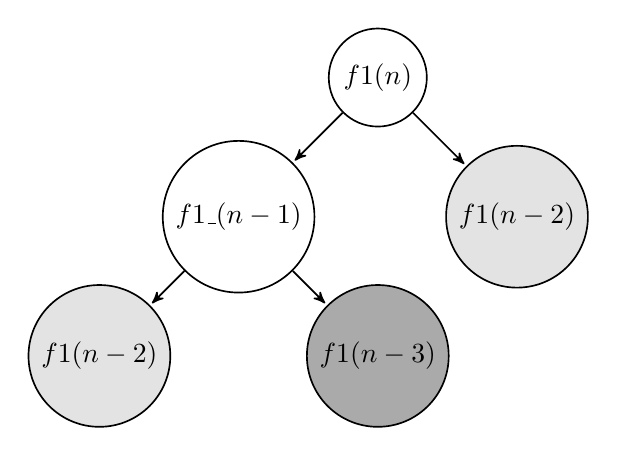
\begin{tikzpicture}[>=stealth',shorten >=1pt,node distance=2.5cm,on grid,semithick]
\tikzstyle{n2} = [circle,draw=black,fill={rgb:black,1;white,8}]
\tikzstyle{n3} = [circle,draw=black,fill={rgb:black,3;white,6}]
    \node[state] (f1n) {$f1(n)$};
    \node[state] (f1n1) [below left =of f1n] {$f1\_(n-1)$};
    \node[n2] (f1n2) [below right =of f1n] {$f1(n-2)$};
    \node[n2] (f1n22) [below left =of f1n1] {$f1(n-2)$};
    \node[n3] (f1n3) [below right =of f1n1] {$f1(n-3)$};
    
    \tikzset{mystyle/.style={->}}
    \tikzset{every node/.style={fill=white}}
    \draw (f1n) edge [mystyle]  (f1n1);
    \draw (f1n) edge [mystyle]  (f1n2);
    \draw (f1n1) edge [mystyle]  (f1n22);
    \draw (f1n1) edge [mystyle]  (f1n3);
\end{tikzpicture}
\end{minipage}
\hspace{5cm}
\begin{minipage}{.2\textwidth}
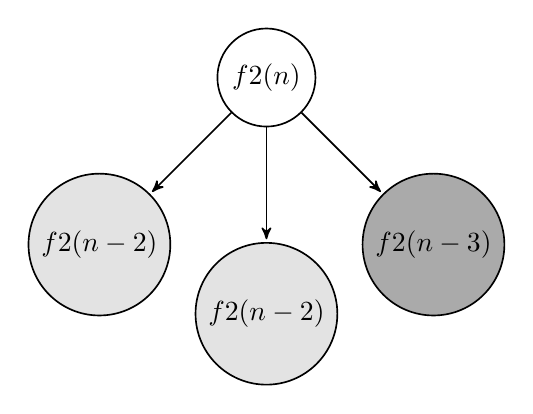
\begin{tikzpicture}[>=stealth',shorten >=1pt,node distance=3cm,on grid,semithick ]
\tikzstyle{n2} = [circle,draw=black,fill={rgb:black,1;white,8}]
\tikzstyle{n3} = [circle,draw=black,fill={rgb:black,3;white,6}]
    \node[state] (f1n) {$f2(n)$};
    \node[n2] (f1n2) [below  =of f1n] {$f2(n-2)$};
    \node[n2] (f1n22) [below left =of f1n] {$f2(n-2)$};
    \node[n3] (f1n3) [below right =of f1n] {$f2(n-3)$};
    
    \tikzset{mystyle/.style={->}}
    \tikzset{every node/.style={fill=white}}
    \draw (f1n) edge [mystyle]  (f1n2);
    \draw (f1n) edge [mystyle]  (f1n22);
    \draw (f1n) edge [mystyle]  (f1n3);
\end{tikzpicture}
\end{minipage}
\caption{The call graphs of $f1$ and $f2$ after unrolling $f1(n-1)$ once. Related calls are colored respectively.}
\label{fig:f1f2cgunrolled}
\end{figure}

Unlike the sum example in figure \ref{fig:sum}, multiple recursive calls in one iteration may require more complex unrollings and thus create a call graph where base cases and $UF$s can each be reached on different levels. The $UFs\_count < 2$ limit works when addressing recursions with a simple step which contains a single recursive call, because it assumes that when $UFs\_count \geq 2$ all the recursive calls on both sides are reached and the model checker can compare the related calls. Dealing with multiple recursive calls nullify this assumption and will fail with a counterexample which holds for $UFs\_count \geq 2$ but does not necessarily reach the same $UF$s on both sides as we have seen in the Fibonacci example above for $n = 2$.

\subsection{A Proof Rule for Simple Step Recursions With Multiple Recursive Calls}
\label{sec:adaptstep}
Before delving into the proof rule itself, we will cover the issues it has to address to overcome the challenges that SEP-PART-EQ had with multiple recursive calls.

Firstly, As seen in the example in figure \ref{fig:f1f2}, we ought to use a differential unrolling, i.e. unroll each recursive call differently, when dealing with multiple recursive calls.

Secondly, The proof for the step case has to include only the inputs that reach all the recursive calls, otherwise it will fail as we have seen in the last example.

Thirdly, due to the last two issues, a gap is created between the input set of the base case, and the input set of the step case after it was unrolled. For example, consider the pair of functions in figure \ref{fig:g1g2neq}.
\begin{figure}[h]
\begin{center}
\begin{minipage}{7 cm}
\begin{lstlisting}
int g1(int n){
   if (n < 1) return 0;
   if (n == 1) return 1; 
   return g1(n-1) + g1(n-2);
}
\end{lstlisting}
\end{minipage}
\begin{minipage}{7 cm}
\begin{lstlisting}
int g2(int n){
   if (n < 1) return 0;
   if (n == 1) return 1; 
   return g2(n-2) + g2(n-2) + g2(n-3) ;
}
\end{lstlisting}
\end{minipage}
\caption{$g1$ and $g2$ diverge on $n=2$.}
\label{fig:g1g2neq}
\end{center}
\end{figure}
$g2$ diverges from $g1$ on $n=2$ as $g1(2) = 1$, and $g2(2) = 0$. In fact $g1$ and $g2$ are not equivalent for \{$n | n = 2 \wedge n \geq 4$\}. BASE-EQUIV$(g1,g2)$ will cover the inputs in $in_B(g1) \cup in_B(g2) = {n \leq 1}$. A step-case proof that considers the first two issues, as stated above, sync-unrolls the call $g1(n-1)$ once, and modifies the condition of the $UFs\_count$ to reach all six recursive calls (2 were created by unrolling $g1(n-1)$). It is easy to see that only for $n \geq 3$ all the recursive calls are reached. As we can see, $n = 2$ was left unproved and has to be addressed to maintain soundness. 

One may suggest addressing the gap set by applying the sync-unrolling before executing the BASE-EQUIV proof. The problem with this method is that the gap traces might not reach any of the original base cases of both programs, as we can see in the example in figure \ref{fig:g1g2neq} for $n=2$. By blocking the recursive calls on each side, BASE-EQUIV prunes all the inputs that do not reach a base case on at least one side, including the gap's traces, and therefore this attempt is futile.
Nevertheless, we can extend the core idea of BASE-EQUIV to accomplish this as well. Essentially, BASE-EQUIV consists of two phases. In each phase RVT blocks the recursive calls of the relevant side and thus left only with the traces that reach this side's base cases. Then, RVT unrolls the other side until equivalence  is proven or timeout is reached. The first part of each phase is used to restrict the input space, and the other part is driven from the understanding that the base cases of equivalent functions are not so far apart, i.e., they require a small amount of unwinding to be proven equivalent. This method could work to prove equivalence for the gap set, but we need to adjust the restriction to include the gap's inputs as well. To do so we will apply the sync-unrolling and generate the base case preconditions of both programs (described in section \ref{sec:findsyncunrolling}), and their disjunction is the constraint that includes the input of the gap case and the base case (note that this is not necessarily the $Weakest\ Precondition$ \cite{10.1145/360933.360975} as the path predicates from the concolic execution may contain redundant clauses). \crjs{this is actually the wp as it is defined semantically regardless to the number of clauses it uses}
Hereafter, we will use the term $Extended\ Base\ Cases$ to state all the traces that reach the base cases and the gap cases combined. 

We propose here a new proof rule MRC-PART-EQ. We will elaborate on the premises EXT-BASE-EQUIV and MRC-STEP-EQUIV in the next sections.
\begin{equation}
 {\frac {\text{EXT-BASE-EQUIV}(f_1,f_2) \:\text{MRC-STEP-EQUIV}(f_1,f_2)}{\text{PARTIAL-EQUIV}(f_1,f_2)}} 
  (\text{MRC-PART-EQ})
\end{equation}

Given a unrolling \emph{su} that synchronizes the functions, (EXT-BASE-EQUIV) prove the conditional equivalence for the extended base case, whereas (MRC-STEP-EQUIV) prove the equivalence of the the step cases. We will now present our method to automatically generate such an unrolling, and then move on to describe (EXT-BASE-EQUIV) and (MRC-STEP-EQUIV).


\section{Automatic synchronization of recursive functions}
%\subsection{The Need To Automatically Synchronize Functions}
To prove equivalence for recursive functions, RVT needs to unroll them so they will be in sync. The motivation for automating the process of finding such an unrolling is clear, and will become even more evident later in the chapter when we consider more complicated cases, in which more involved rules will be presented, for functions with multiple recursive calls. 

As stated before, RVT replaces all the recursive calls with $UF$s. If the functions are out of sync, the calls to the uninterpreted functions with different arguments result in different return values, which fails the proof.

Consider the functions $f1$ and $f2$ from figure \ref{fig:f1f2}.
They are not in sync as $f1$ reaches two recursive calls with the parameters: $n-1,n-2$, while $f2$ reaches calls with $n-2,n-2,n-3$ as arguments and thus the calls are not \emph{related}.
\begin{definition}[Related Calls]
\label{def:relatedcalls}
Given two functions $f$ and $f'$, two recursive calls of $f$ and $f'$ respectively are \emph{related}  if they are called with equivalent arguments.  
\end{definition}
The call graphs of this pair can be seen in figure \ref{fig:f1f2cgs}.

\begin{figure}
\begin{minipage}{.2\textwidth}
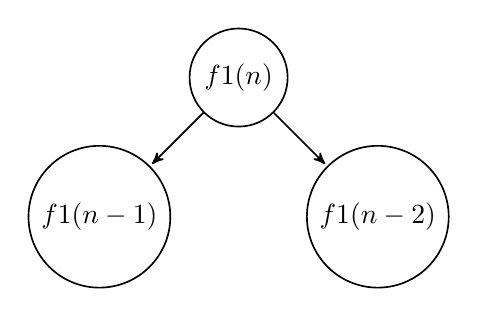
\begin{tikzpicture}[>=stealth',shorten >=1pt,node distance=2.5cm,on grid,semithick ]
\tikzstyle{uf} = [circle,draw=black,fill={rgb:black,1;white,8}]
    \node[state] (f1n) {$f1(n)$};
    \node[state] (f1n1) [below left =of f1n] {$f1(n-1)$};
    \node[state] (f1n2) [below right =of f1n] {$f1(n-2)$};

    
    \tikzset{mystyle/.style={->}}
    \tikzset{every node/.style={fill=white}}
    \draw (f1n) edge [mystyle]  (f1n1);
    \draw (f1n) edge [mystyle]  (f1n2);
\end{tikzpicture}
\end{minipage}
\hspace{5cm}
\begin{minipage}{.2\textwidth}
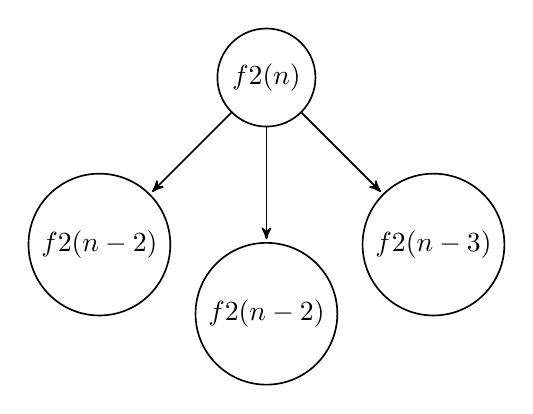
\begin{tikzpicture}[>=stealth',shorten >=1pt,node distance=3cm,on grid,semithick ]
\tikzstyle{uf} = [circle,draw=black,fill={rgb:black,1;white,8}]
    \node[state] (f1n) {$f2(n)$};
    \node[state] (f1n2) [below  =of f1n] {$f2(n-2)$};
    \node[state] (f1n22) [below left =of f1n] {$f2(n-2)$};
    \node[state] (f1n3) [below right =of f1n] {$f2(n-3)$};
    
    \tikzset{mystyle/.style={->}}
    \tikzset{every node/.style={fill=white}}
    \draw (f1n) edge [mystyle]  (f1n2);
    \draw (f1n) edge [mystyle]  (f1n22);
    \draw (f1n) edge [mystyle]  (f1n3);
\end{tikzpicture}
\end{minipage}
\caption{The call graphs of f1 and f2 from figure \ref{fig:f1f2}.}
\label{fig:f1f2cgs}
\end{figure}
Clearly, $f1$ and $f2$ are out of sync. However, unrolling the call of $f1(n-1)$ once solves this problem: see figure \ref{fig:f1f2unrolled}. As in~\cite{DBLP:conf/fm/StrichmanV16} unrolling is done by creating a new function $f1\_$ that has an identical body as $f1$ and replacing the call to $f1(n-1)$ with $f1\_(n-1)$.

\begin{figure}[h]
\begin{center}
\begin{minipage}{7 cm}
\begin{lstlisting}
int f1_(int n){
   if (n < 1) return 0;
   if (n == 1) return 1; 
   return f1(n-1) + f1(n-2);
}

int f1(int n){
   if (n < 1) return 0;
   if (n == 1) return 1; 
   return f1_(n-1) + f1(n-2);
}
\end{lstlisting}
\end{minipage}
\begin{minipage}{7 cm}
\begin{lstlisting}
int f2(int n){
   if (n < 1) return 0;
   if (n <= 2) return 1;
   return f2(n-2) + f2(n-2) + f2(n-3) ;
}
\end{lstlisting}
\end{minipage}
\caption{Unrolling the call to $f1(n-1)$ keeps the semantic behaviour of the original $f1$.}
\label{fig:f1f2unrolled}
\end{center}
\end{figure}
 Unrolling a recursion keeps the original functionality of the program and thus soundness is preserved. The call graphs of the unrolled program can be seen in figure \ref{fig:f1f2cgunrolled}. 

After applying the unrolling, both programs are in sync, or, more formally: 
\begin{definition}[Sync-Unrolling]
An unrolling \emph{su} of two recursive functions $f$ and $f'$ is called \emph{Sync-Unrolling} if after applying it all the recursive calls on each side have related calls on the other side.
\end{definition}

More generally, call graphs of recursions might have a more complicated pattern that will require to unroll several levels of the recursions on either side in order to achieve such synchronisation. Also, calls can be conditioned, which means that the correct unrolling depends on the input value. Furthermore, it is possible to construct examples of two equivalent recursive functions that no unrolling makes them synchronise. We will discuss this later in the chapter. 

We now describe a method for finding sync-unrolling when possible.

\subsection{Finding the sync-unrolling}
Our method, described in algorithm \ref{alg:Findunrolling}, finds an input to the functions and corresponding sync-unrolling $su$, if such an unrolling exists. Of course, we can also force the input to a given value or range. For functions $f$,$f'$ with a simple control flow (as the Fibonacci implementations in figure \ref{fig:f1f2}), a single unrolling is sufficient, whereas for others a domain partitioning is necessary. This issue is discussed in section \ref{sec:multistep} . 

Consider figure \ref{fig:f1f2cgunrolled}, where $f1$ is unrolled once. The leaves of the two call graphs can be pairwise matched to one another, such that a matched pair represents related calls. To find such an unrolling automatically, we create a C program for CBMC, that its counterexample represents the unrolling numbers per function call site. The main idea is that we let CBMC decide whether to make a recursive call or not, and record the parameters where it decides not to make a recursive calls (these will be the leaves of the call graph, where we will call the uninterpreted functions). We assert that at least one recorded parameter on both sides is different, and hence a counterexample that CBMC finds is an input to the functions, and an unrolling in which all parameters are equal under this input. 

\begin{definition}[Simple Step]
A step case of a recursion is called a \emph{Simple Step} if its control flow contains a single path.
\end{definition}
Our method finds an unrolling for a specific input rather than for the general case of the recursion. But, if the recursion's step case is a simple step, then we can induce that unrolling is a sync-unrolling for any input of the step case.
The overall algorithm appears in the next subsection. 

\subsection{An Algorithm To Find sync-unrollings} \label{sec:findsyncunrolling}
Consider Algorithm \ref{alg:Findunrolling}. Its main functions are: 
\begin{itemize}
    \item \alg{AddDepthAndCallsTracking}$(f)$ adds the auxiliary infrastructure needed to record the exact call graph of a given counterexample. This is done by adding the depth and the recursive call site (i.e. each recursive is given an index according to their order of appearance in the function) to the functions calls so CBMC could show them when producing the counterexample.
    \item \alg {GetBaseCasePrecondition}$(f)$ computes the base case precondition $bcpc$ that needs to hold in order for no recursive calls to be taken in $f$. This is done as follows. All recursive calls are replaced with call to  functions that has a single line: assume(false). Then RVT uses $Concolic\ Execution$, a method introduced by Sen in \cite{10.1145/1321631.1321746} and implemented in PathCrawler  by Williams et al. \cite{10.1007/11408901_21}, to generate the paths predicates of the feasible paths. The paths with the recursive calls are all blocked and as a result this process will produce the path predicates of the base cases. Since this is a flat program (no loops and recursions), this is guaranteed to terminate with a correct answer.
    \item \alg{AddAssumption}$(f,p)$ assumes the precondition $p$ at the beginning of $f$. 
    \item \alg{ApplyNonDeterministicRecording}$(f)$ adds a non-deterministic condition after the assumption on the base case. If that condition holds, the input of this iteration is recorded and the function aborts. Otherwise it has no effect. Considering the call graphs of a pair that is unrolled with sync-unrolling, this method is meant to simulate the leaves on those graphs. For finding the sync-unrolling, we care about their arguments, and whether they had recursive calls or not is irrelevant.
    \item \alg{CreateSyncUnrollingVerificationProgram}$(f_1,f_2)$ generates a new programs that combines the programs into a single program $P$ by renaming similar identifiers, generating a non deterministic input and feeding it to both programs. Then, after the calls to $f_1$ and $f_2$, it asserts that the non-empty sets of recorded inputs from \alg{ApplyNonDeterministicRecording} are never equal.
\iffalse    
    as shown in figure \ref{fig:findcutverfprogram}.
  \begin{figure} [h]
\begin{center}
\begin{minipage}{7 cm}
\begin{lstlisting}[escapeinside={(*}{*)}]
i = non_det()
input_set(*$_1$*) = input_set(*$_2$*) = {}
res1 = (*$f_1$*)(i)
res2 = (*$f_2$*)(i)
assume(input_set(*$_1$*).size > 1 && input_set(*$_2$*).size > 1)
assert(input_set(*$_1$*) != input_set(*$_2$*))
\end{lstlisting}
\end{minipage}
\caption{The program $P$ generated in line~\ref{step:create} of Algorithm~\ref{alg:Findunrolling}. There is an input\_set array for each variable $f_1$ and $f_2$ receives as input.}
\label{fig:findcutverfprogram}
\end{center}
\end{figure}
  \fi
\item \alg{CBMC}$(P)$ is the call to the model checker CBMC that will either prove the assertions in $P$ as correct or generate a counterexample.
\item \alg{GenerateSynchronizingUnrolling}$(f_1,f_2,ce)$ uses the information from \alg{AddDepthAndCallsTracking} to generate the sync-unrolling by extracting which call should be unrolled on each iteration and how many times. 
\end{itemize}  

\noindent
\begin{algorithm}
\begin{minipage}{\linewidth}
\begin{algorithmic}[1]
\Function{FindSyncUnrolling}{Loops Free Programs $f_1,f_2$}
    \For { $ i \in \{1,2\}$}\label{step:foreach_p} \label{step:setupforsu}
    \State $f_i$ = \alg{AddDepthAndCallsTracking}$(f_i)$\label{step:depth_tracking}
    \State $bcpc$ = \alg{GetBaseCasePrecondition}$(f_i)$\label{step:get_bcpc}
    \State $f_i$ = \alg{AddAssumption}$(f_i,!bcpc)$\label{step:block_bc}
    \State $f_i$ = \alg {ApplyNonDeterministicRecording}$(f_i)$
    \EndFor
    \State $P$ = \alg{CreateSyncUnrollingVerificationProgram}$(f_1,f_2)$\label{step:create}
    \For{unwinding factor $uw$ increasing from 1 up until a predefined timeout}
        \State $P_{unwinded}$ = \alg{Unwind}$(P,uw)$
        \If {CBMC$(P_{unwinded})$ results with a counterexample $ce$}
        \State \Return \alg{GenerateSynchronizingUnrolling}$(f_1,f_2,ce)$
        \EndIf
    \EndFor
\EndFunction
\end{algorithmic}
\end{minipage}
\caption{An algorithm to find an unrolling for two programs that will synchronize them.}
\label{alg:Findunrolling}
\end{algorithm}

We will demonstrate the method on the pair from figure \ref{fig:f1f2}. After applying the setup in the for loop in line \ref{step:setupforsu}, $f_1$ and $f_2$ are transformed to the pair in figure \ref{fig:f1f2susetup}.
\begin{figure}[h]
\begin{center}
\begin{lstlisting}
int f1(int n, int depth, int recursive_call_site){
    assume(n > 1);
    if(non_det()){
        recorded_n1[recorded_n_size1++] = n;
        return NULL;
    }
    if (n < 1) return 0;
    if (n == 1) return 1; 
    return f1(n-1) + f1(n-2);
}

int f2(int n, int depth, int recursive_call_site){
    assume(n > 2);
    if(non_det()){
        recorded_n2[recorded_n_size2++] = n;
        return NULL;
    }
    if (n < 1) return 0;
    if (n <= 2) return 1;
    return f2(n-2) + f2(n-2) + f2(n-3) ;
}
\end{lstlisting}
\caption{$f1$ and $f2$ after the setup loop in line \ref{step:setupforsu}. $recorded\_n1$, $recorded\_n\_size1$, $recorded\_n2$, $recorded\_n\_size2$ are all global variable. The size variables are initialized to 0 and are needed for the C implementation that CBMC verifies when asserting the equivalence of the recorded inputs.}
\label{fig:f1f2susetup}
\end{center}
\end{figure}

Then, the program $P$ generated in line \ref{step:create} is shown in figure \ref{fig:findcutverfprogramf1f2}.
\begin{figure} [h]
\begin{center}
\begin{minipage}{7 cm}
\begin{lstlisting}
i = non_det()
recorded_n1 = recorded_n2 = {}
recorded_n_size1 = recorded_n_size2 = 0
f1(i,0,-1)
f1(i,0,-1)
assume(recorded_n_size1 > 0 && recorded_n_size2 > 0)
assert(recorded_n1 != recorded_n2)
\end{lstlisting}
\end{minipage}
\caption{The program $P$ generated in line~\ref{step:create} of Algorithm~\ref{alg:Findunrolling} for $f1$ and $f2$ from figure \ref{fig:f1f2susetup}}
\label{fig:findcutverfprogramf1f2}
\end{center}
\end{figure}

After unwinding $P$ enough times CBMC will find a counterexample for any n bigger than 2, from which \alg{GenerateSynchronizingUnrolling} derives the sync-unrolling shown in figure \ref{fig:f1f2cgunrolled}.


\section{EXT-BASE-EQUIV - Proving Extended Base Cases Equivalence}
\label{sec:EXT-BASE-EQUIV}
To prove EXT-BASE-EQUIV, RVT generates a verification program that represents the equivalence we want to prove. The composition of such a program is depicted in algorithm  \ref{alg:ExtendedBaseProof}.

\noindent
\begin{algorithm}
\begin{minipage}{\linewidth}
\begin{algorithmic}[1]
\Function{ProveExtendedBaseCasesProof}{ Programs $f_1,f_2$, sync-unrolling $su$}
    \For { $ i \in \{1,2\}$}\label{step:foreach_p}
	\State$\bar{f_i}$ = \alg{ApplyUnrolling}($f_i$,$su$)
	\State $bcpc_i$ = \alg{GetBaseCasePrecondition}$(\bar{f_i})$
	\EndFor
	\State $P$ = \alg{CreateVerificationProgram}$(\bar{f_1},\bar{f_2})$
    \State $P$ = \alg{AddAssumption}($P$,$bcpc_1 \lor bcpc_2$) \label{step:assumebcpc12}
    \State $P$ = \alg{AddEquivalenceAssertion}($P$)
    \State return \alg{SymbolicExecution}($P$)
	\EndFunction
\end{algorithmic}
\end{minipage}
\caption{A sound algorithm to prove equivalence of programs for their extended base cases.}
\label{alg:ExtendedBaseProof}
\end{algorithm}
The sync-unrolling $su$ is provided by using the method described in algorithm \ref{alg:Findunrolling}. Note that $su$ have an unrolling instruction for each program and also that those programs are loop free as RVT converts all loops to recursions in an earlier stage. After applying $su$ to both programs, a base case precondition is generated for each program with \alg{GetBaseCasePrecondition} as explained in section \ref{sec:findsyncunrolling}. Those preconditions will be used later to restrict the proof to address only the extended base case. RVT calls \alg{CreateVerificationProgram} that combines the programs into a single program $P$ by renaming similar identifiers, generating a non deterministic input and feeding it to both programs. Line \ref{step:assumebcpc12} assumes $bcpc_1 \lor bcpc_2$ at the beginning of $P$ to limit the proof to the extended base case (the complementary formula represent the inputs that reach no base case on either side, which is the step case). At last, equivalence is asserted. A schematic depiction of $P$ is shown in figure \ref{fig:basegapvefprogram}. 
\begin{figure} [h]
\begin{center}
\begin{minipage}{7 cm}
\begin{lstlisting}[escapeinside={(*}{*)}]
i = non_det()
assume((*$bcpc_1 \lor bcpc_2$*))
res1 = (*$\bar{f_1}$*)(i)
res2 = (*$\bar{f_2}$*)(i)
assert(res1==res2)
\end{lstlisting}
\end{minipage}
\caption{A verification program to prove conditional equivalence for the extended base cases.}
\label{fig:basegapvefprogram}
\end{center}
\end{figure}
In fact, we restrict the notation of equivalence to conditional equivalence as Kawaguchi et al. described in their work in \cite{kawaguchi2010conditional}. That is, to prove the equivalence for the extended base cases we will prove the equivalence of the pair only on inputs that satisfy $bcpc_1 \lor bcpc_2$. Symbolic Execution is used to verify $P$. If the verification task is successful then RVT will deem the extended base case equivalence of the pair as correct. 

\subsection{Comparing methods to prove the extended base cases equivalence}
We choose to use the Symbolic Execution method to prove the extended base cases equivalence due to complexity reasons. We will compare here the complexity of two alternatives. The first is using CBMC and increasing the unrolling factor until the verification is successful or timeout is reached. The second is using Symbolic Execution. It is important to note that we aim to compare the method's asymptotic complexity rather than their exact complexity, and the discussion will be held accordingly.  

Assume that we try to prove the said equivalence of two programs $P_1$ and $P_2$ and that at least one of them contains two or more recursive calls in its body that are executed on the same trace. Let $C$ be that number. Without loss of generality, assume that the equivalence is proved when $P_1$ is unrolled $k$ times. Therefore we can conclude that $C > 1$ and $k \geq 0$. Let $n$ be the syntactic size of $P_1$ and $P_2$ that includes their variables and functions. 

One can think of it as if the method that involves CBMC invokes the SAT solver only one time after traversing the whole call graph, which is a tree as we unroll the recursions, while the second method is running in a DFS form on the call graph and calls the SAT solver every time it reaches a leaf.

If we were to use CBMC, the unrolling would create a program that is translated to a formula that its size is bounded by $O(C^k{\cdot}n)$. To understand this claim, consider the call graph of such a pair. An example can be seen in figure \ref{fig:f1f2cgunrolled}. As one can observe, the call graph expands as a tree where each vertex has a number of edges that is equal to the number of recursive calls taken in the step case. There might be of course more edges due to other calls. The amount of nodes in such a tree is $O(C^k)$. The encoding to a propositional formula creates a different set of variables for every call, and thus the formula's size has the order of $O(C^k{\cdot}n)$. CBMC calls a SAT solver to solve this formula, and SAT is known to be an NP-complete problem. Hence the complexity for the verification task is exponential in $O(C^k{\cdot}n)$, thus the complexity of this method is in the order of double exponential in the span of the recursive calls.
%$O(C_0^{Poly(n)})$ where $Poly(n)$ is a polynomial of $n$, and $C_0$ is a constant. Thus, the complexity is: \[ O(C_0^{Poly({C^k{\cdot}n})}) \]

On the other hand, using Symbolic Execution, the size of the formula is bounded by $O(k{\cdot}n)$ as it represents only a single trace. Symbolic Execution goes through all paths up to a given bound, and the the number of paths is worst-case exponential (this is the known ``path explosion" problem  \cite{10.1007/978-3-540-78800-3_28}). Each of these trace verification tasks is a formula handed to a SAT solver and therefore has an exponential run-time bound. That means that the overall complexity of this method is exponential squared in the program's size. 
Hence using symbolic execution for this task has better performances than the CBMC based method mentioned above.


\section{MRC-STEP-EQUIV - Proving Step Case Equivalence}
\label{sec:MRC-STEP-EQUIV}
\noindent
\begin{algorithm}
\begin{minipage}{\linewidth}
\begin{algorithmic}[1]
\Function{ProveStepCaseEquivalence}{ Programs $f_1,f_2$, sync-unrolling $su$, precondition $ebcp$}
	\State$\bar{f_1}$ = \alg{ApplyUnrolling}($f_1$,$su$)
	\State$\bar{f_2}$ = \alg{ApplyUnrolling}($f_2$,$su$)
	\State $P$ = \alg{CreateVerificationProgram}$(\bar{f_1},\bar{f_2})$
	\State $P$ = \alg{ReplaceRecursionsWithUFs}$(P)$
	\State $P$ = \alg{AddAssumption}($P,!ebcp$)
    \State $P$ = \alg{AddEquivalenceAssertion}($P$)
    \State return \alg{CBMC}($P$)
	\EndFunction
\end{algorithmic}
\end{minipage}
\caption{A sound algorithm to prove equivalence of programs for their extended base cases.}
\label{alg:StepCaseProof}
\end{algorithm}
The step-case proof tries to prove the general case for inputs that are not contained in the extended base case set. In the step case, after applying sync-unrolling, if an input's trace reaches only related recursive calls then we can say that the pair is equivalent for the step case. Algorithm \ref{alg:StepCaseProof} describes RVT's process to do so.
\alg{ProveStepCaseEquivalence} receives the sync-unrolling $su$ that is provided by using the method described in algorithm \ref{alg:Findunrolling}. It also receives the extended base case precondition $bcpc_1 \lor bcpc_2$ that is generated in algorithm \ref{alg:ExtendedBaseProof} and is aliased here as $ebcp$. As we portrayed the requirements for the step-case proof in section \ref{sec:adaptstep}, we refined the input space to include only step case inputs by using the negation of $bcpc_1 \lor bcpc_2$. The key element of this proof is replacing all the recursive calls that are left after applying $su$ with $UF$s. The reason we can do so is because the important thing for this proof is whether all the recursive calls have related calls. The proof is agnostic to the body of those calls and therefore they can be replaced with $UF$s. As $f_1$ and $f_2$ are loop-free and after applying \alg{ReplaceRecursionsWithUFs} $P$ is also recursion free, the verification task of $P$ is simplified to verify a flat program with no need of unwinding. $P$ is presented in figure \ref{fig:stepvefprogram}. $\hat{f_i}$ stands for the function $f_i$ after being unrolled and the recursive calls replaced with $UF$s. If CBMC validate $P$ then we know the pair is step-case equivalent. 
\begin{figure} [h]
\begin{center}
\begin{minipage}{7 cm}
\begin{lstlisting}[escapeinside={(*}{*)}]
i = non_det()
assume(!ebcp)
res1 = (*$\hat{f_1}$*)(i)
res2 = (*$\hat{f_2}$*)(i)
assert(res1==res2)
\end{lstlisting}
\end{minipage}
\caption{A verification program using $ebcp$ derived from algorithm \ref{alg:ExtendedBaseProof} to prove conditional equivalence for the step case.}
\label{fig:stepvefprogram}
\end{center}
\end{figure}

\subsection{The soundness of MRC-PART-EQ}
\label{sec:MRCsoundness}
In EXT-BASE-EQUIV, RVT tries to prove equivalence for all the traces that do not reach a recursive call on one of the functions. In MRC-STEP-EQUIV, RVT tries to prove equivalence for the complementary group of EXT-BASE-EQUIV's inputs. By definition, EXT-BASE-EQUIV's and MRC-STEP-EQUIV's input domain cover together all the possible inputs. MRC-PART-EQ requires both EXT-BASE-EQUIV and MRC-STEP-EQUIV to be equivalent for the proof to hold, and hence it is sound.


\section{Proving Equivalence For Complex Step Recursions}
\label{sec:multistep}
\subsection{Applying MRC-PART-EQ on Complex Step Recursions}
For the following discussion we will first define what is a complex step recursion:
\begin{definition}[Complex Step]
The step case of a recursion is a \emph{Complex Step} if its control flow contains two or more paths.
\end{definition}
Let's examine the recursions in figure \ref{fig:f1f2cond}.
\begin{figure}[h]
\begin{center}
\begin{minipage}{7 cm}
\begin{lstlisting}
int h1(int n){
   if (n < 1) return 0;
   if (n == 1) return 1; 
   return h1(n-1) + h1(n-2);
}
\end{lstlisting}
\end{minipage}
\begin{minipage}{7 cm}
\begin{lstlisting}
int h2(int n){
   if (n < 1) return 0;
   if (n == 1) return 1; 
   if (n & 1 == 0)
        return h2(n-1) + h2(n-2);
   if (n & 1 == 1)
        return h2(n-2) + h2(n-2) + h2(n-3);
}
\end{lstlisting}
\end{minipage}
\caption{Equivalent implementations of Fibonacci, whereas h2 has a complex step. $n \& 1$ check the parity of $n$ using the AND bitwise operation.}
\label{fig:f1f2cond}
\end{center}
\end{figure}
For $n\leq 1$ both functions behave the same. For $n=2$, $n$ is even and thus the same related recursive calls are executed on both sides. As we have seen in the example from figure \ref{fig:f1f2}, for $n\geq3$ the two possible steps are interchangeable for calculating the Fibonacci sequence. Nevertheless, MRC-PART-EQ cannot find a useful sync-unrolling to prove equivalence for this pair, because in fact here a different unrolling is necessary for different traces.
\os{show here how partitioning of the domain, each with its own sync-unrollings, solves this problem, for this example. }
In the next subsection we will show how to partition the domain such that each partition induces a single trace of the program, thus solving this problem. 

\os{consider whether the following is necessary:}
Furthermore, to compute the base-case precondition for the extended base case in EXT-BASE-EQUIV, we heavily rely on the total recursive calls coverage due to the assumption that the step case is the path where all those calls are invoked, and anything below is the gap case or the base case. This assumption is dismissed when dealing with complex steps, as no trace can reach all the recursive calls in a single path.

\subsection{Proving equivalence of complex-step recursive functions}
Given two functions as described in the previous subsection, we would like to decompose them to multiple functions such that each of them has a simple step. We will then prove the equivalence of each such pair of functions. For this purpose we will use path predicates to divide the input domain. Formally, let $CF(f)$ be the set of all the paths in the control flow of the top frame of a function $f$. Let $in(p)$ denote all the inputs that their traces go through the path $p$, $f|_a$ denote the function $f$ with an assumption $a$ restricting its inputs, and $base(f_1,f_2)=in_B(f_1) \cup in_B(f_2)$ ($in_B(f)$ was described in section \ref{sec:prev}).
Based on this notation, we define the proof rule CS-PART-EQ:

\begin{equation}
{\frac{
  \bigwedge_{p_1\in CF(f_1)}\bigwedge_{p_2\in CF(f_2)}\text{MRC-PART-EQ}(f_1|_{base(f_1,f_2) \cup in(p_1)},f_2|_{base(f_1,f_2) \cup in(p_2)})}{\text{PARTIAL-EQUIV}(f_1,f_2)}}\text{(CS-PART-EQ)}
\end{equation}
If we omit the base cases ($base(f_1,f_2)$), either EXT-BASE-EQUIV and BASE-EQUIV would have been vacuously true for any path of the step cases. By including the base cases to each pair of step cases we can use MRC-PART-EQ without any changes and sustain its soundness. CS-PART-EQ covers all the possible pairs of paths, and due to its exhaustive nature and the fact that for each pair of recursions MRC-PART-EQ is sound (as shown in \ref{sec:MRCsoundness}), we can conclude that CS-PART-EQ is sound as well.

\begin{algorithm}
\begin{minipage}{\linewidth}
\begin{algorithmic}[1]
\Function{ProveComplexStepsRecursions}{ Functions $f_1,f_2$}
    \State $AreEquivalent$ = TRUE
    \For { $ i \in \{1,2\}$}\label{step:foreach_p}
	\State \label{step:getallpaths} $PathsPredicates_i$ = \alg{GetAllPAths}$(f_i)$
	\State \label{step:GetBaseCasePrecondition} $pp_{f_{base}^i}$ = \alg{GetBaseCasePrecondition}($f_i$) 
	\EndFor
	\For{every pair <$pp_1,pp_2$> in $PathsPredicates_1 \times PathsPredicates_2$}
	\If{ $ pp_1 \cap pp_2 = \emptyset$} \label{step:skip_unfeasible}
	\State continue
	\EndIf
	\State \label{step:addassumption} $f_{pruned}^1$ = \alg{AddAssumption}($f_1$, $pp_1\lor pp_{f_{base}^1}$) 
	\label{step:assmp1}
	\State $f_{pruned}^2$ = \alg{AddAssumption}($f_2$, $pp_2 \lor pp_{f_{base}^2}$) 
	\label{step:assmp2}
	\State su = \alg{FindSyncUnrolling}($f_{pruned}^1$,$f_{pruned}^2$)
	\State $BaseCaseEquiv$ = \alg{ProveExtendedBaseCasesProof}($f_{pruned}^1,f_{pruned}^2,su$) 
	\State \label{step:provestepincs} $StepCaseEquiv$ = 	\alg{ProveStepCaseEquivalence}($f_{pruned}^1,f_{pruned}^2,su,bcpc_1\lor bcpc_2$)
 \If{ \label{step:false}
	(!( BaseCaseEquiv $\wedge$ StepCaseEquiv)}
	\State \Return FALSE; 
	\EndIf
	\EndFor
    \State \Return TRUE;
	\EndFunction
\end{algorithmic}
\end{minipage}
\caption{A sound algorithm to prove equivalence for complex step recursions.}
\label{alg:provemcr}
\end{algorithm}

Algorithm~\ref{alg:provemcr} shows 
\alg{ProveComplexStepsRecursions}, which checks the premise of CS-PART-EQ. It partitions the input domain of the two input functions, such that each partition corresponds to a separate path in their flattened version, as explained above. It then tries to prove the equivalence of each pair of such partitions. The main elements of the algorithm are: 
\begin{itemize}
    \item In line~\ref{step:getallpaths},
    \alg{GetAllPaths($f$)} uses \emph{concolic execution} to get all the paths in the top frame of $f$. To that end, \alg{GetAllPaths} flattens $f$ by replacing recursive calls with calls to empty functions, i.e., functions that have a single $return$ statement and nothing else, and calls PathCrawler \cite{10.1007/11408901_21}. PathCrawler generates a list of path conditions for all the possible paths in that flattened version of $f$.  
    \item In line~\ref{step:GetBaseCasePrecondition} \alg{GetBaseCasePrecondition} is called. It is the same as the one described in section \ref{sec:findsyncunrolling}.
    \item In line \ref{step:skip_unfeasible} we screen out infeasible paths, as a performance optimization. It is based on the observation that some of the paths predicates combinations in $PathsPredicates_1 \times PathsPredicates_2$ are not feasible. RVT checks this by creating a verification task as presented in figure \ref{fig:checkfeasibility}. In the generated program, we assume both path predicates on the same non deterministic inputs. Sending this task to a model checker results in two option: $1.$ If the verification is successful, that means the conjunctions of the assumptions is unsatisfiable and thus the intersection of $pp_1$ and $pp_2$ is empty. $2.$ If the verification fails, that means the paths in question are feasible as the verification reaches the false assertion.
    
    \item As of line~\ref{step:addassumption}, for each feasible pair of paths predicates, RVT treats the programs as though they had a single step by restricting the inputs and tries to prove them with \alg{ProveExtendedBaseCasesProof} and \alg{ProveStepCaseEquivalence} from sections \ref{sec:EXT-BASE-EQUIV} and \ref{sec:MRC-STEP-EQUIV}, respectively. \alg{AddAssumption} in those algorithms deviates from how is was originally described. Rather than just adding the assumptions, it replaces the assumptions added in algorithm \ref{alg:provemcr} in lines~\ref{step:assmp1} and~\ref{step:assmp2}. Otherwise, when blocking the base cases for example, we will assume contradicting assumptions and the verification task would be vacuously true. The formula $bcpc_1\lor bcpc_2$ in line \ref{step:provestepincs} is computed as part of  \alg{ProveExtendedBaseCasesProof} in the line above. 
    
    \item In line~\ref{step:false}, we return False (i.e., we failed proving that $f_1$ and $f_2$ are equivalent), if we failed proving equivalent one of the pairs. 
\end{itemize}

\begin{figure} [h]
\begin{center}
\begin{minipage}{7 cm}
\begin{lstlisting}[escapeinside={(*}{*)}]
i = non_det()
assume(*($pp_1(i)$*) && (*($pp_2(i)$*))
assert(false)
\end{lstlisting}
\end{minipage}
\caption{A verification task for checking   the emptiness of an intersection of two input domains, which are defined by the path predicates $pp_1$ and $pp_2$ over an input argument $i$.}
\label{fig:checkfeasibility}
\end{center}
\end{figure}

\subsection{A demonstration of the incompleteness of CS-PART-EQ}
Although CS-PART-EQ can prove a range of use cases with multiple parameters and various variables types, in this section we will discuss some of its limitations.
\begin{figure}[h]
\begin{center}
\begin{minipage}{7 cm}
\begin{lstlisting}
int m1(int n, int do_nothing) {
    if (n < 1) return 0;
    if (n == 1) return 1;
    return m1(n - 1, !do_nothing) 
    + m1(n - 2, !do_nothing);
}
\end{lstlisting}
\end{minipage}
\begin{minipage}{7 cm}
\begin{lstlisting}
int m2(int n, int switch_mode) {
    if (n < 1) return 0;
    if (n == 1 || n == 2) return 1;
    int results = 0;
    if (switch_mode)
        results = m2(n - 2,!switch_mode) 
        + m2(n - 2,!switch_mode) 
        + m2(n - 3, !switch_mode);
    if (!switch_mode)
       results = m2(n - 1, !switch_mode) 
       + m2(n - 2, !switch_mode);
    return results;

}
\end{lstlisting}
\end{minipage}
\caption{Equivalent implementations of Fibonacci. m2 alternates between two paths in the control flow.}
\label{fig:f1f2switch}
\end{center}
\end{figure}


1. Consider the pair in figure \ref{fig:f1f2switch}. As we have seen throughout this chapter, the steps are equivalent for $n > 3$ and $n=2$ is handled in m2's base case and so this pair is equivalent. For the case where switch\_mode is true, RVT generates a sync-unrolling that unrolls the call m1(n-1,!do\_nothing) once, as we would expect. When trying to prove the related step case, CBMC will fail. This happens because in the added unrolled frame the polarity of do\_nothing is negated to the polarity of switch\_mode in the related calls due to the odd number of unrolling, and as a consequence there won't be related uninterpreted functions that the SAT solver could compare, even though that do\_nothing does not affect m1 results.

Talk about:
1. Switch case example
2. Redundant recursive calls that defect the sync-unrolling generation
3. Mutual recursion






































\iffalse
\noindent
\begin{algorithm}
\begin{minipage}{\linewidth}
\begin{algorithmic}[1]
\Function{ProveEquivalenceWithUnrolling}{sync-unrolling su, Programs $f,f'$}
	\State$(\bar{f},\bar{f'})$ = apply unrolling on f and f'
	\If{\alg{BASE-EQUIV}$(\bar{f},\bar{f'})$ is EQUIVALENT $\wedge$
		   \alg{GAP-EQUIV}$(\bar{f},\bar{f'})$ is EQUIVALENT 	$\wedge$
		   \alg{STEP-EQUIV}$(\bar{f},\bar{f'})$ is EQUIVALENT}
	\State	return EQUIVALENT
	\Else
	\State	return NOT EQUIVALENT
		\EndIf
	\EndFunction
\end{algorithmic}
\end{minipage}
\caption{A sound algorithm to prove equivalence for programs with multiple recursive calls given a synchronisation unrolling}
\label{alg:ProveWithUnrolling}
\end{algorithm}
   
   
   \noindent
\begin{algorithm}
\begin{minipage}{\linewidth}
\begin{algorithmic}[1]
\Function{ProveEquivalence}{Programs $f,f'$}
	\State sync-unroll = \alg{FindSynchronizingUnrolling}($f,f'$)
	\If{sync-unroll != NULL}
	\State	return \alg{ProveEquivalenceWithUnrolling}(sync-unroll,$f,f'$)
	\Else
	\For{every unrolling of $f,f'$ (advance gradually until timeout is reached)}
	\State$(\bar{f},\bar{f'})$ = unroll(sync-unroll,$f,f'$)
	\If{\alg{STEP-EQUIV}(sync-unroll,$\bar{f},\bar{f'}$) is EQUIVALENT $\wedge$
	{\alg{BASE-EQUIV}$(\bar{f},\bar{f'})$ is EQUIVALENT $\wedge$ \alg{GAP-EQUIV}(sync-unroll,$\bar{f},\bar{f'}$) is EQUIVALENT}}
		   \State return EQUIVALENT
	
	\EndIf
	\EndFor
	\EndIf
	\State return NOT EQUIVALENT
\EndFunction
\end{algorithmic}
\end{minipage}
\caption{A sound algorithm to prove equivalence for programs with multiple recursive calls}
\label{alg:WholesomeProve}
\end{algorithm}
\fi

\chapter{Tools integration to improve completeness}
\label{chptr:integ}
\section{Improving Completeness Using Tools Integration}
The first contribution of my research is to integrate RVT and REVE and by doing so produce a technique that is more complete than each one of them on its own. More specifically, the new algorithm will be able to prove equivalence for at least each case RVT or REVE could. The feature that let us to combine both engines is the doom mechanic we have described is section \ref{sec:rvtreview}. One of its advantages is that it let us integrate other tools into the decomposition process. We would like to use REVE in three cases. The first is when RVT fails, REVE will be invoked and will try to prove equivalence for the same pair. The second is when we encounter a doomed function in the call graph that has a mapping to a function in the second program. That means that one of its descendants was a recursive function and could not be proven equivalent to any other function in the second program. As we said, this nullifies RVT capability of proving equivalence. As stated in section \ref{sec:relatedwork}, REVE works differently and isn't affected by this limit. Hence, if we execute REVE on the pair, and it will succeed, we will note both functions and their ancestors as not doomed. From this pair and upward in the call graph, RVT can be used again. The third case is when a node is doomed due to lack of mapping. The problem here lies in the mapping algorithm used to generate the input for RVT decomposition algorithm. Once the algorithm fails to map a recursive function it stops trying to map its ancestors as well. This made sense when the only proof engine was RVT, but now it has become an obstacle we must overcome. A new mapping algorithm needs to be chosen, one that can map ancestors even in the case their descendants could not be mapped. A trivial solution could be mapping all the functions with the same signature. I will experiment whether this idea can hold in real life programs or perhaps a more sophisticated idea must be conceived. Once we have figured a way to expand our mapping, REVE will be able to check for their equivalence. And as in the second case, if it succeeds, we will be able to execute RVT from hereon. 

The combined algorithm is shown in Algorithm \ref{alg:Prove}. It receives the mapping as input, and therefore is agnostic to our mapping generation algorithm. There are several key changes it is important to note. In line \ref{step:whileOneSide} we iterate over MSCC nodes in one graph rather than mapping pairs as in Algorithm \ref{alg:OldProve}. That is because the original algorithm assumed the mapping must be \emph{connected} - every mapped pair is either a map between leaves in the call graphs or the children of both paired functions are mapped as well. We want to allow now an \emph{unconnected} mapping – pair of functions that their descendants are not necessarily mapped. Iterating over such a mapping is achieved by traversing only one call graph. Because the mapping relation is symmetric, and each pair contains a node from this call graph, it is assured we will cover all the pairs in the mapping. Another significant change is the addition of "RVT enable" which helps to track for each MSCC whether RVT can be invoked to check its equivalence to its mapped MSCC. This flag is updated throughout Algorithm \ref{alg:Prove} repetitively in the cases that were described earlier in this section.  

\noindent
\begin{algorithm}
\begin{minipage}{\linewidth}
\begin{algorithmic}[1]
\Function{Prove}{Programs $P,P'$, map between functions $map_f$}
\State \label{step:inline} Inline nonrecursive nonmapped functions;
\State \label{step:generate} Generate MSCC DAGs $MD_1$, $MD_2$ from the call graphs of $P, P′$; 
\State \label{step:markEnabled} mark all the nodes in $MD_1$ as "RVT enabled";
\State If possible, generate a bijective map $map_m$ between nontrivial nodes in $MD_1$ and $MD_2$ that is consistent with \mbox{~~~~~} $map_f$ (it is desirable but not necessary to add pairs of trivial nodes to $map_m$). Otherwise Abort. 
\While {$\exists m1 \in MD_1$ that is uncovered, and its children are “Covered”} \label{step:whileOneSide}
\If {$\exists m2 \in MD_2\ s.t.\ \exists \pair{m1,m2} \in map_m $} \label{step:findMapping}
   \If {$m,m'$ are trivial} \label{step:m1}
     \State Let $f,f'$ be the functions in $m,m'$, respectively;
     \If {\alg{$check^r$}$(m1,f,f',\{\pair{f,f'}\})$} \label{step:Check}
      \alg{markEquivalent}$(f1, f2, m1)$; \label{step:markTrivial}
    \EndIf
   \Else
    \label{step:select} 
    \State Select non-deterministically $S \subseteq \{\pair{f,f'}\mid \pair{f,f'}\in map_f(m)\}$ \newline \mbox{~~~~~~~~~~~~~~~~~~~~~~~} that intersect every cycle in $m1$ and $m2$;
      \For {each $ \pair{f,f'} \in S$}\label{step:forall}
        \If  {$\lnot \alg{check^r}(m1,f,f',S)$} \label{step:abort}
         \State Mark m1 and all its ancestors as not "RVT enabled"; \label{step:doom}
        \State Break;
        \EndIf
      \EndFor
      \If {m1 is marked "RVT enabled"} \label{step:markNonTrivial}
      \For {each $ \pair{f,f'} \in S$}\ {\alg{MarkEquivalent}$(f1, f2, m1)$}
      \EndFor
      \EndIf
      \EndIf
      \Else
      \If {m1 is not trivial }
      \State Mark m1 and all its ancestors as not "RVT enabled";
      \EndIf
   \EndIf
   \State Mark m1 as “Covered”;
\EndWhile
\EndFunction
\end{algorithmic}
\end{minipage}
\caption{A decomposition algorithm integrating RVT and REVE}
\label{alg:Prove}
\end{algorithm}
\begin{algorithm}
\begin{minipage}{\linewidth}
\begin{algorithmic}[1]
\Function {$Check^r$}{$MSCC\  m1,function\ f, function\ f′, set\ of\ pairs\ S$}
\label{step:Checkr2}
\If{m1 is marked as "RVT enabled" }
\If{f and f′ are syntactically equivalent and all their children are either marked “Equivalent” or in S }
\State \Return true;
\EndIf
\If{CBMC ($Check-block^r$(f,f′,S))}
\State \Return true;
\EndIf
\EndIf
\State Let $S_{equal}$ be the set of all the functions proved equal so far in our execution
\State \Return LLREVE$(f,f',S_equal)$
\EndFunction
\end{algorithmic}
\end{minipage}
\caption{A function called by \alg{Prove} for checking the equivalence of two input functions that are part of MSCCs. This version execute both proving engine - RVT and REVE. $check-block^r$ is the same C program as in the old \alg{$check^r$}.}
\end{algorithm}
\begin{algorithm}
\begin{minipage}{\linewidth}
\begin{algorithmic}[1]
\Function {MarkEquivalence}{function f, function f′, MSCC m}
\label{step:markEquivalent}
\State Mark f1 and f2 as "Equivalent";
\State Mark m1 as "RVT enabled"; 
\For{each ancestor g of m1 in }
\If{all the sons of g are marked as "RVT enabled" }
\State Mark g as "RVT enabled";
\EndIf
\EndFor
\EndFunction
\end{algorithmic}
\end{minipage}
\caption{A function called from \alg{Prove} to mark the equivalence of $m1$ and its mapping in $MD_2$.}
\end{algorithm}

\begin{figure}
\label{fig:callgraphs}
\begin{center}
\begin{minipage}{.2\textwidth}
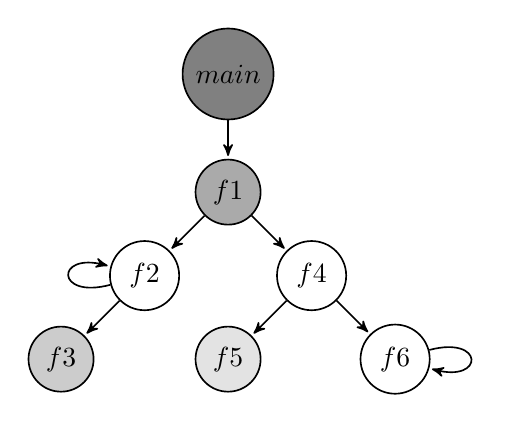
\begin{tikzpicture}[>=stealth',shorten >=1pt,node distance=1.5cm,on grid,semithick ]
\tikzstyle{mapped0} = [circle,draw=black,fill={rgb:black,2;white,2}]
\tikzstyle{mapped1} = [circle,draw=black,fill={rgb:black,1;white,2}]
\tikzstyle{mapped2} = [circle,draw=black,fill={rgb:black,1;white,4}]
\tikzstyle{mapped3} = [circle,draw=black,fill={rgb:black,1;white,8}]
    \node[mapped0] (main) {$main$};
    \node[mapped1] (f1) [below =of main] {$f1$};
    \node[state] (f2) [below left =of f1] {$f2$};
    \node[state] (f4) [below right =of f1] {$f4$};
    \node[mapped2] (f3) [below left =of f2] {$f3$};
    \node[mapped3] (f5) [below left =of f4] {$f5$};
    \node[state] (f6) [below right =of f4] {$f6$};
    
    \tikzset{mystyle/.style={->}}
    \tikzset{every node/.style={fill=white}}
    \draw (main) edge [mystyle]  (f1);
    \draw (f1) edge [mystyle]  (f2);
    \draw (f1) edge [mystyle]  (f4);
    \draw (f2) edge [loop left]  (f2);
    \draw (f2) edge [mystyle]  (f3);
    \draw (f4) edge [mystyle]  (f5);
    \draw (f4) edge [mystyle]  (f6);
    \draw (f6) edge [loop right]  (f6);
\end{tikzpicture}
\end{minipage}
\hspace{3.5cm}
\begin{minipage}{.2\textwidth}
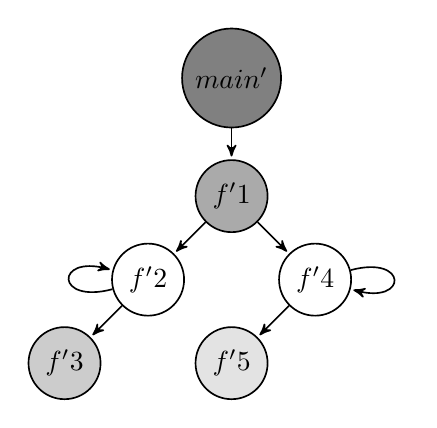
\begin{tikzpicture}[>=stealth',shorten >=1pt,node distance=1.5cm,on grid,semithick ]
\tikzstyle{mapped0} = [circle,draw=black,fill={rgb:black,2;white,2}]
\tikzstyle{mapped1} = [circle,draw=black,fill={rgb:black,1;white,2}]
\tikzstyle{mapped2} = [circle,draw=black,fill={rgb:black,1;white,4}]
\tikzstyle{mapped3} = [circle,draw=black,fill={rgb:black,1;white,8}]
    \node[mapped0] (main') {$main'$};
    \node[mapped1] (f'1) [below =of main'] {$f'1$};
    \node[state] (f'2) [below left =of f'1] {$f'2$};
    \node[state] (f'4) [below right =of f'1] {$f'4$};
    \node[mapped2] (f'3) [below left =of f'2] {$f'3$};
    \node[mapped3] (f'5) [below left =of f'4] {$f'5$};
    
    \tikzset{mystyle/.style={->}}
    \tikzset{every node/.style={fill=white}}
    \draw (main') edge [mystyle]  (f'1);
    \draw (f'1) edge [mystyle]  (f'2);
    \draw (f'1) edge [mystyle]  (f'4);
    \draw (f'2) edge [loop left]  (f'2);
    \draw (f'2) edge [mystyle]  (f'3);
    \draw (f'4) edge [mystyle]  (f'5);
    \draw (f'4) edge [loop right]  (f'4);
  
\end{tikzpicture}
\end{minipage}
\end{center}
\caption{$MD_1$ and $MD_2$. Mapped nodes are colored with their unique grey. }
\end{figure}

We will now show an example where \alg{Prove} (Algorithm \ref{alg:Prove}) achieves better results in term of completeness than \alg{OldProve} (\ref{alg:OldProve}). 
\begin{example}
Consider $MD_1$ and $MD_2$ in Figure \ref{fig:callgraphs}. $map_m$ is defined as $map_m = \{ \pair{main,main'},\pair{f1,f'1}, \pair{f3,f'3},\pair{f5,f'5}\}$. Note that $map_m$ is an \emph{unconnected} mapping ($\pair{f1,f'1}$ have no mapped sons) and could not be generated by RVT before applying the changes we have proposed here. \alg{OldProve} from Algorithm \ref{alg:OldProve} would have faced two problems when checking equivalence for this example. First, it would have stopped when it has finished checking equivalence for $\pair{f3,f'3}$ and $\pair{f5,f'5}$. After covering those pairs, \alg{OldProve} cannot find any pair that is uncovered and its children are "Covered" and will terminate its execution. Our new \alg{Prove} from Algorithm \ref{alg:Prove} resolves this issue by traversing only $MD_1$. Every node in $MD_1$ will be visited and will be checked for equivalence against its pair in $MD_2$ if exists. The second problem exists even after changing the traversing algorithm of \alg{OldProve}. Once it has reached $f6$ it would have aborted. That is because RVT cannot handle an equivalence checking of functions where one of its children is recursive and is not equivalent to any other function in the other program. In \alg{Prove}, encountering $f6$ would doom all its ancestors, but it will not abort as LLREVE will be used to check their equivalence. In our example, $f4$ will be encountered but it has no mapping so no check will be performed here. Next, $f1$ will be visited, and because it is mapped to $f'1$, LLREVE will be executed to check their equivalence. For the sake of this example let us assume it has succeeded. Now that all the recursive children of main are equivalent (i.e. $f1$), $main$ will be undoomed and RVT can be used to check the equivalence of $\pair{main,main'}$. Those two virtues of \alg{Prove} over \alg{OldProve} are a major step forward towards a more complete generator for proofs of equivalence .
\end{example}

\bibliographystyle{plain}  
\bibliography{references}

\end{document}
